\subsection{Rubric-Score Rankings as a Robustness Check}
\label{app:rubric-score-ranking}

Our primary rankings use pairwise win rates. Because each judge also assigns
dimension-level rubric scores to both responses, we construct a second set of
rankings directly from those scores. This analysis tests whether the reported
model ordering depends on converting judgments into binary pairwise outcomes,
or whether a similar ordering emerges from the underlying micro-rubric
evaluations.

We retain both signals because they answer complementary evaluation questions.
Comparative judgment asks which of two outputs is better and can preserve
holistic differences that are difficult to encode exhaustively in advance.
Rubric scoring instead decomposes quality into explicit task-specific and
general dimensions, making the source of a model's strengths and weaknesses
inspectable. Recent evidence from expert legal evaluation finds that pairwise
comparisons recover an intended quality ordering more accurately, and in less
annotation time, than absolute rubric scoring in that setting
\citep{yang2026judgmentbench}. At the same time, rubric scores provide a
transparent diagnostic record that a winner alone cannot supply. Rubric-based
LLM evaluation can itself be sensitive to score-option ordering and scale use
\citep{xu2026pointwisepairwise}, which further motivates treating standardized
rubric rankings as a complementary robustness analysis rather than replacing
the comparative outcome.

We construct the score-based rankings separately within each run. First, for
every model--task--mode--judge cell, we average the task-specific and general
rubric dimensions, giving each dimension equal weight. Judges differ in how
they use the 1--10 scale, so we standardize these averages within each
run--task--mode--judge comparison universe. We then average standardized
scores across the judges eligible under the leave-family-out rule and rank
models within each run, task, and mode. Finally, we average these ranks across
the ten runs and report their standard errors. Ranking models within each run
before averaging preserves run-to-run variation; directly pooling all scores
across runs produces slightly weaker agreement with the pairwise results.

\begin{figure}[H]
    \centering
    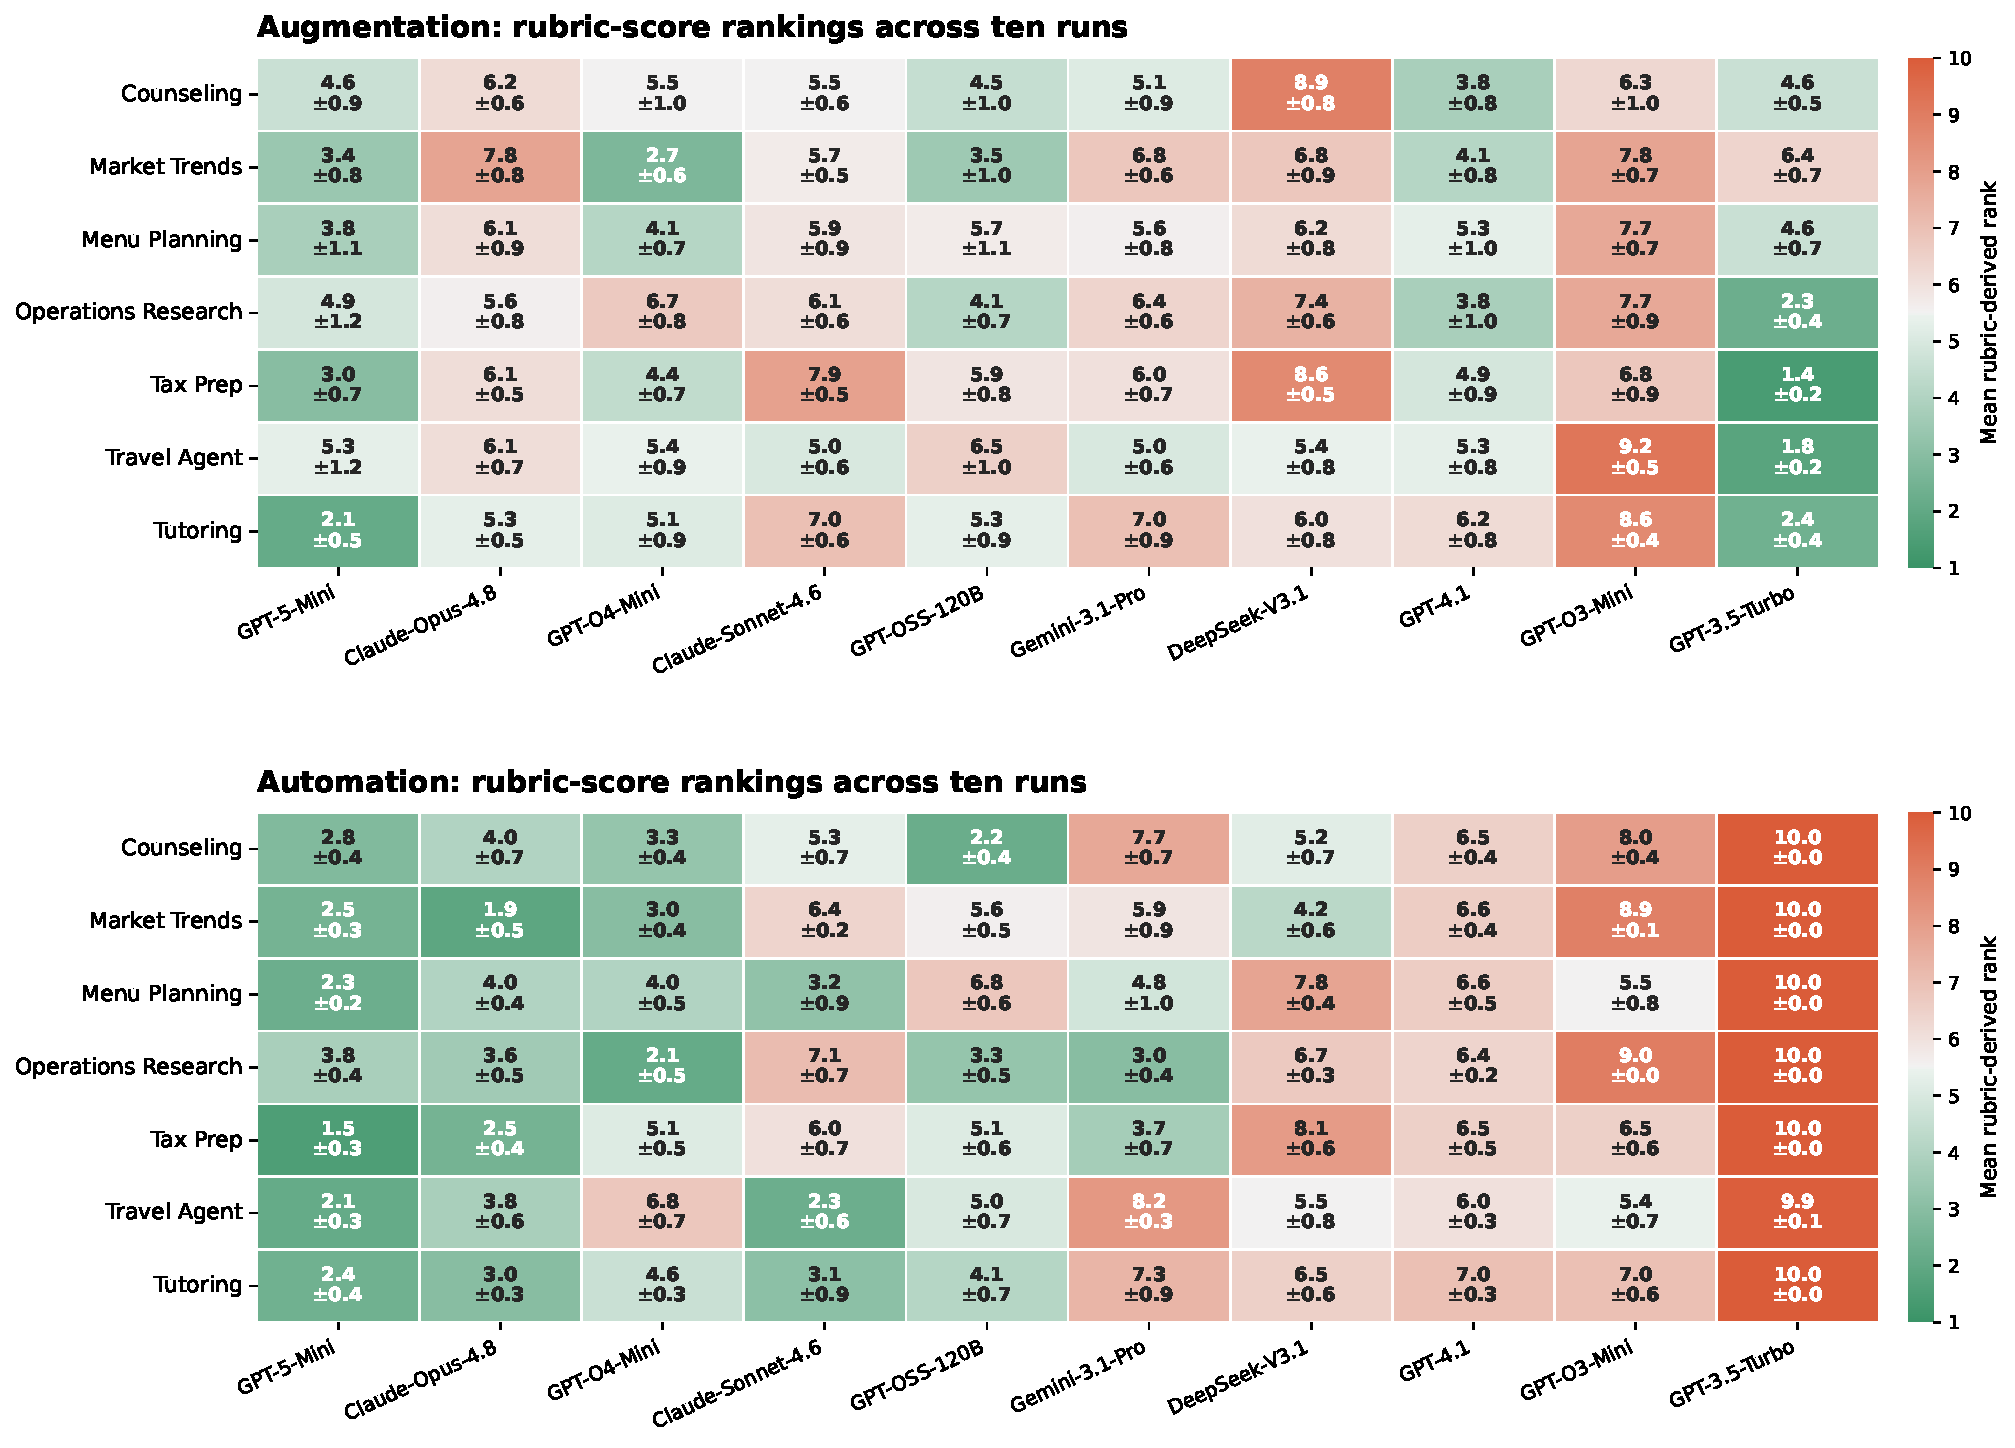
\includegraphics[width=\linewidth]{paper_figures/figureA_rubric_score_rank_heatmaps.pdf}
    \caption{
    Rankings derived from dimension-level rubric scores across ten independent
    runs. Before aggregation, rubric averages are standardized within each
    judge's run--task--mode comparison universe to account for differences in
    scale use. Each cell reports the mean within-run rank, with its standard
    error beneath; lower values indicate better performance. The GPT-3.5-Turbo
    column represents the unaided worker in augmentation and the direct solver
    in automation.
    }
    \label{fig:rubric-score-rankings}
\end{figure}

Figure~\ref{fig:rubric-score-rankings} shows that the rubric-derived rankings
recover the main substantive patterns in the pairwise analysis. Automation is
concentrated around a relatively small group of strong direct solvers, whereas
augmentation remains more task-dependent. The unaided worker remains highly
competitive in several augmentation tasks, and no assistant model leads every
task.

\begin{figure}[H]
    \centering
    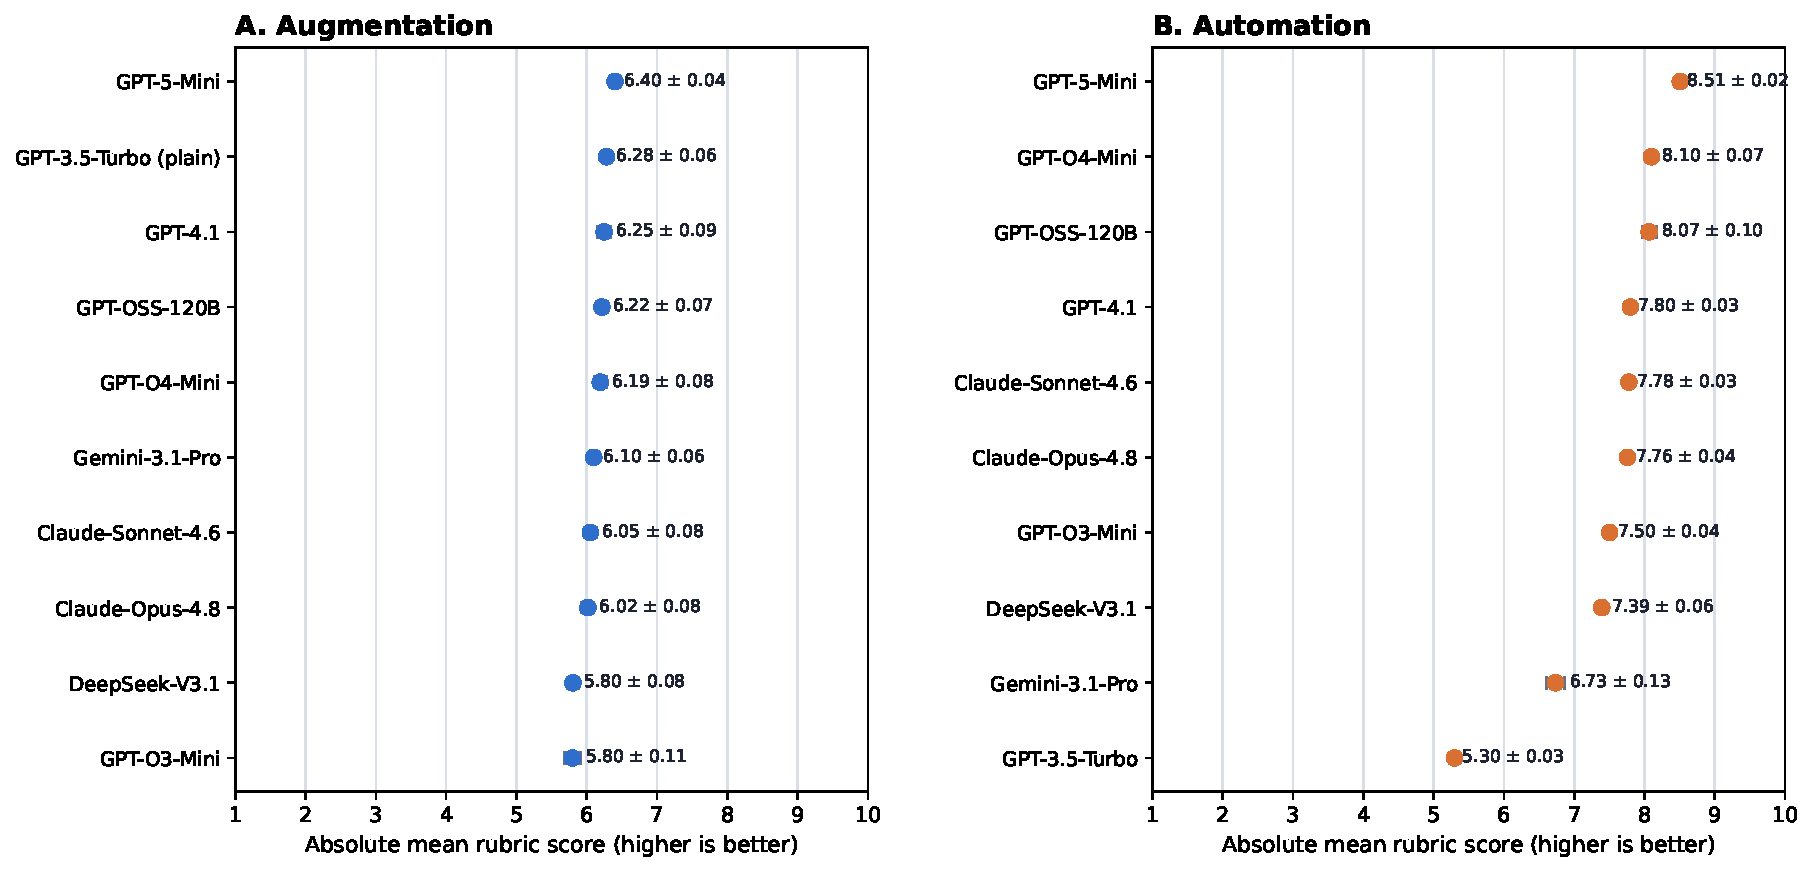
\includegraphics[width=\linewidth]{paper_figures/figureA_model_average_rubric_scores.pdf}
    \caption{
    Absolute mean rubric score by model and regime. Scores are first averaged
    across tasks within each run and then averaged across ten independent runs;
    error bars report standard errors across the ten run-level averages. Higher
    scores indicate better evaluated output quality. In augmentation,
    GPT-3.5-Turbo (plain) denotes the unaided worker. Because absolute scores
    remain sensitive to judge scale use and to the eligible leave-family-out
    judge set, this figure is descriptive; the standardized within-run rankings
    in Figure~\ref{fig:rubric-score-rankings} provide the primary score-based
    robustness comparison.
    }
    \label{fig:absolute-rubric-scores}
\end{figure}

The absolute-score view in Figure~\ref{fig:absolute-rubric-scores} leads to the
same broad conclusion. GPT-5-Mini has the highest mean score in both regimes,
but the augmentation scores are tightly clustered: GPT-5-Mini scores 6.40,
the unaided worker scores 6.28, and GPT-4.1 scores 6.25. Automation separates
models more sharply, with GPT-5-Mini averaging 8.51 compared with 5.30 for
GPT-3.5-Turbo. This difference in dispersion is consistent with the greater
concentration of automation rankings and the more fragmented augmentation
results.

\begin{figure}[H]
    \centering
    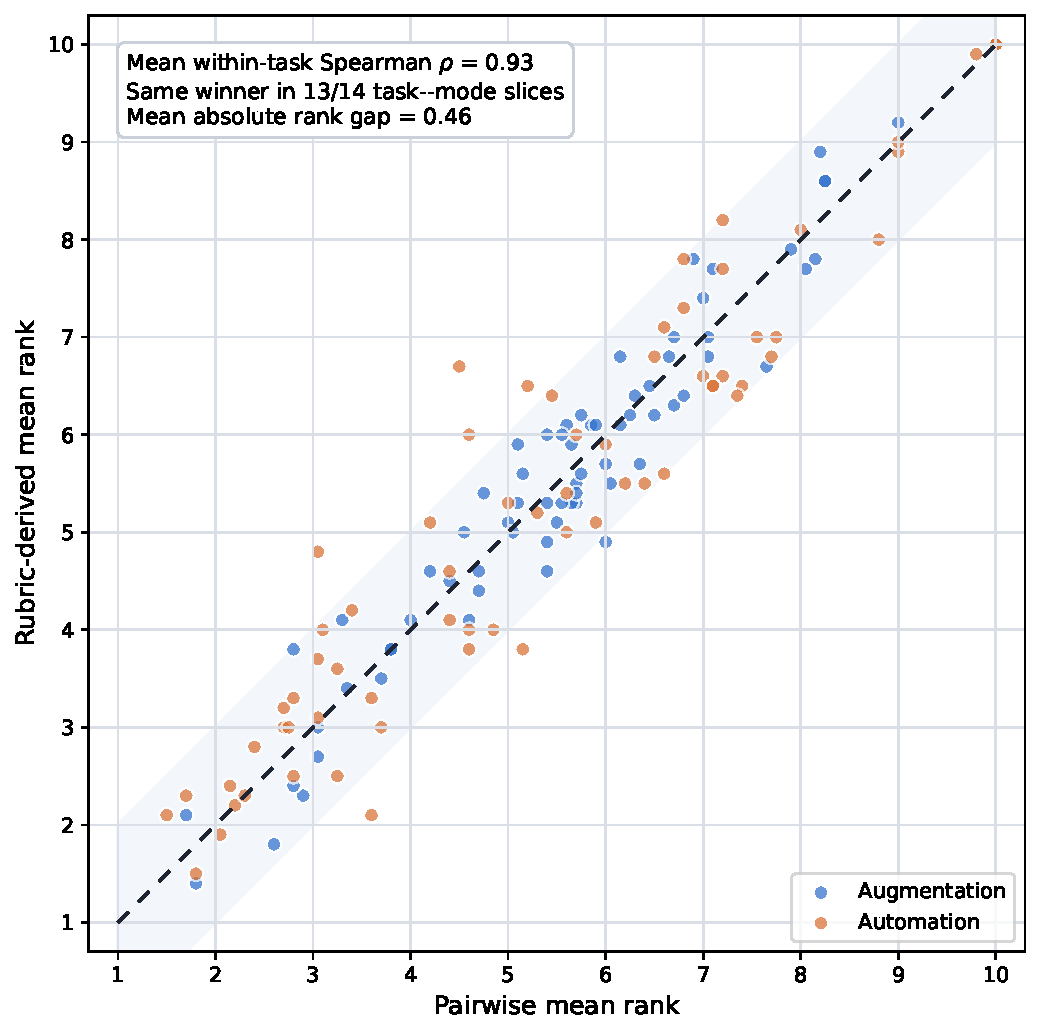
\includegraphics[width=0.78\linewidth]{paper_figures/figureA_pairwise_vs_rubric_rank_alignment.pdf}
    \caption{
    Alignment between pairwise and rubric-derived rankings. Each point is one
    model in one task--mode cell, averaged across ten runs. The dashed
    45-degree line denotes identical ranks, and the shaded region marks a
    difference of at most one rank position. Across the 14 task--mode slices,
    the mean within-slice Spearman correlation is $\rho=0.93$. The two methods
    identify the same top-ranked model in 13 of 14 slices and differ by 0.46
    rank positions on average.
    }
    \label{fig:pairwise-rubric-rank-alignment}
\end{figure}

The two aggregation methods are closely aligned
(Figure~\ref{fig:pairwise-rubric-rank-alignment}). Their mean within-task
Spearman correlation is $0.93$, and they select the same winner in 13 of the
14 task--mode comparisons. The sole winner-level disagreement occurs for
operations-research automation: the pairwise procedure ranks
Gemini-3.1-Pro first, whereas the rubric-score procedure ranks GPT-O4-Mini
first. Across all model--task--mode cells, the mean absolute difference is
0.46 rank positions.

We therefore retain pairwise win rate as the primary comparative outcome for
three reasons. First, a pairwise choice is ordinal and is less dependent on
whether one judge uses, for example, scores of 6--8 while another uses 8--10.
Second, direct comparison can distinguish outputs whose absolute rubric scores
are close and allows a judge to account for a decisive hard-constraint
violation that may be diluted in a simple dimension average. Third, pairwise
evaluation has a direct interpretation as comparative preference and has shown
stronger recovery of expert-intended quality than rubric scoring in at least
one recent high-expertise benchmark \citep{yang2026judgmentbench}. The
rubric-derived rankings remain essential complementary evidence: they expose
which dimensions drive an outcome, preserve the magnitude of score
differences, and provide an auditable diagnostic profile for each model.

This agreement should be interpreted as a robustness check rather than an
independent pointwise validation. In our protocol, the rubric scores and
pairwise choices are produced in the same evaluation call, and the judge sees
both responses while assigning dimension scores. A fully independent pointwise
validation would present each response in isolation to a separate judge panel
and would require additional controls for rubric-scale and option-order bias
\citep{xu2026pointwisepairwise}. Nevertheless, the close correspondence shows
that the headline rankings are not sensitive to whether the same judgments are
aggregated as binary pairwise outcomes or as standardized dimension-level
scores. Pairwise results establish the ordering; rubric results verify that
ordering and explain where the evaluated differences arise.
